\section{Aufgabe 5}
\setcounter{section}{5}

Betrachten Sie die Studienfachwahl von 200 Studienanf"angern an einer
Hochschule. Die Verteilung der Studienanf"anger auf die verschiedenen F"acher
ist wie folgt:

\begin{table}[h]
    \centering
    \begin{tabular}{l|c}
        \multicolumn{1}{l}{Studienfach} & \multicolumn{1}{c}{Anzahl der Studierenden} \\ \hline
        Informatik & 45 \\
        Architektur & 30 \\
        Wirtschaft & 25 \\
        Maschinenbau & 35 \\
        Elektrotechnik & 20 \\
        Lebensmitteltechnik & 25 \\
        Sonstige & 20
    \end{tabular}
    \caption{}
\end{table}

\begin{enumerate}[1.]
    \item Bestimmen Sie die relativen H"aufigkeiten f"ur jedes Studienfach und
        berechnen Sie diese.

        \begin{enumerate}[i)]
            \item $r_{\text{Informatik}} = \dfrac{45}{200} = 0,225$
            \item $r_{\text{Architektur}} = \dfrac{30}{200} = 0,15$
            \item $r_{\text{Wirtschaft}} = \dfrac{25}{200} = 0,125$
            \item $r_{\text{Maschinenbau}} = \dfrac{35}{200} = 0,175$
            \item $r_{\text{Elektrotechnik}} = \dfrac{20}{200} = 0,1$
            \item $r_{\text{Lebensmitteltechnik}} = \dfrac{25}{200} = 0,125$
            \item $r_{\text{Sonstige}} = \dfrac{20}{200} = 0,1$
        \end{enumerate}
    \vspace{10pt}
    \item Erstellen Sie ein Balkendiagramm, das die relativen H"aufigkeiten der
        Studienf"acher visualisiert.

        Siehe Abbildung~\ref{fig:abbildung-05-01}.

    \item Erstellen Sie ein Kreisdiagramm, das die gleichen Daten darstellt.

        Siehe Abbildung~\ref{fig:abbildung-05-02}.

    \item Diskutieren Sie, welches Diagramm geeigneter ist, um die Verteilung
        der Studienfachwahl darzustellen und warum.

        Bei quantitativen Daten stellt das Balkendiagramm die
        Häufigkeit der Werte klarer dar als das Kreisdiagramm,
        weil es die einzelnen Werte entlang einer Achse sichtbar
        macht und Unterschiede in der Höhe der Balken auf einen
        Blick erkennbar sind.

    \begin{figure}[p]
        \centering
        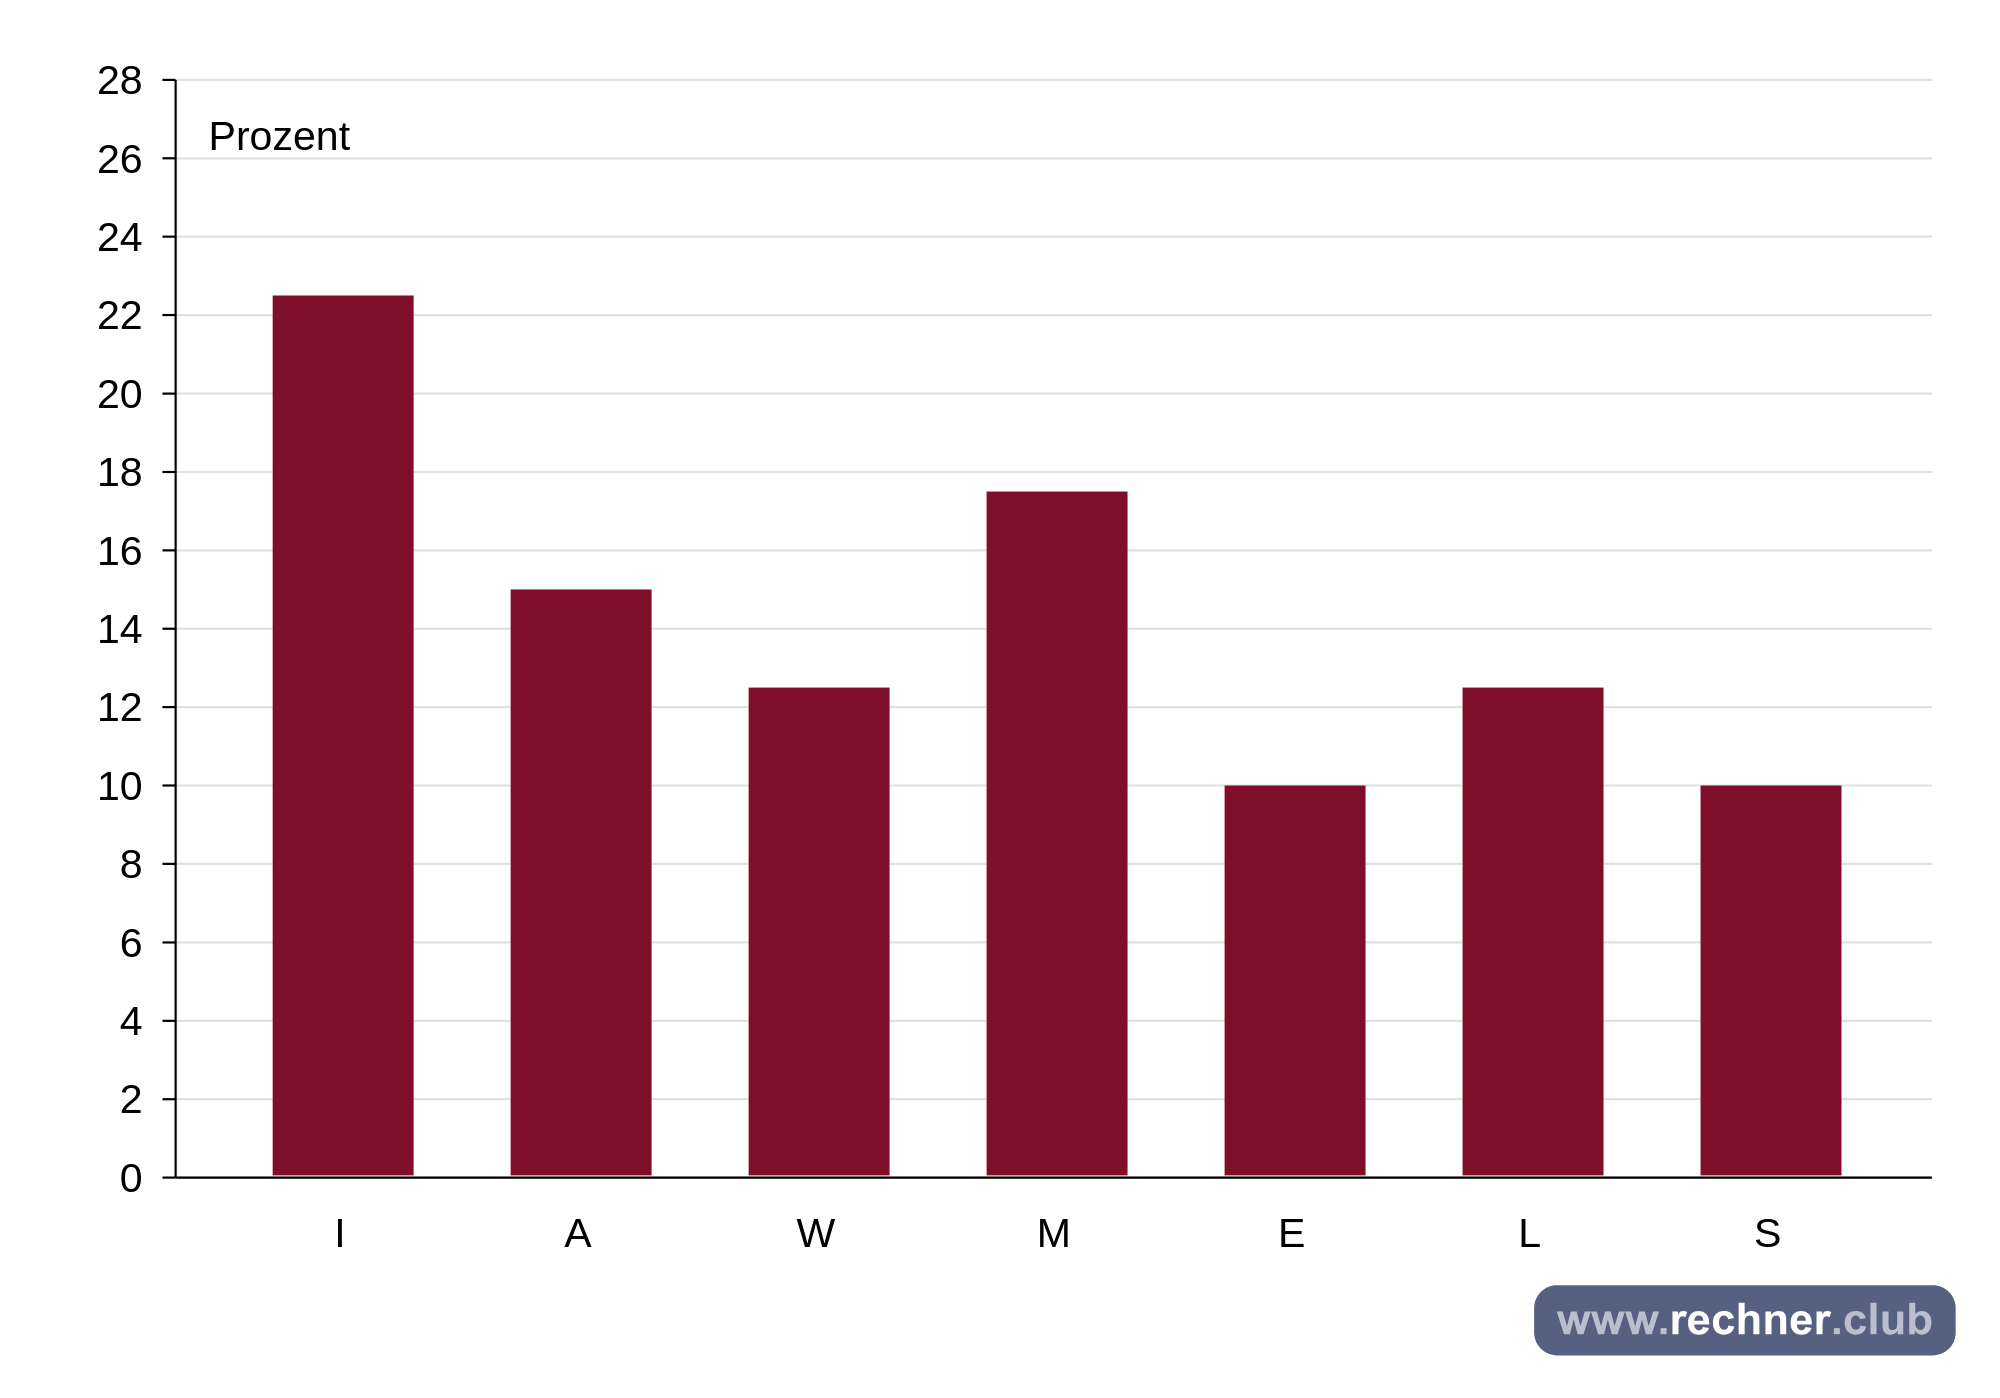
\includegraphics[width=0.8\textwidth]{./assets/abbildung-05-01.png}
        \caption{H"aufigkeit der Studienf"acher (Balkendiagramm)}
        \label{fig:abbildung-05-01}
    \end{figure}

    \begin{figure}[p]
        \centering
        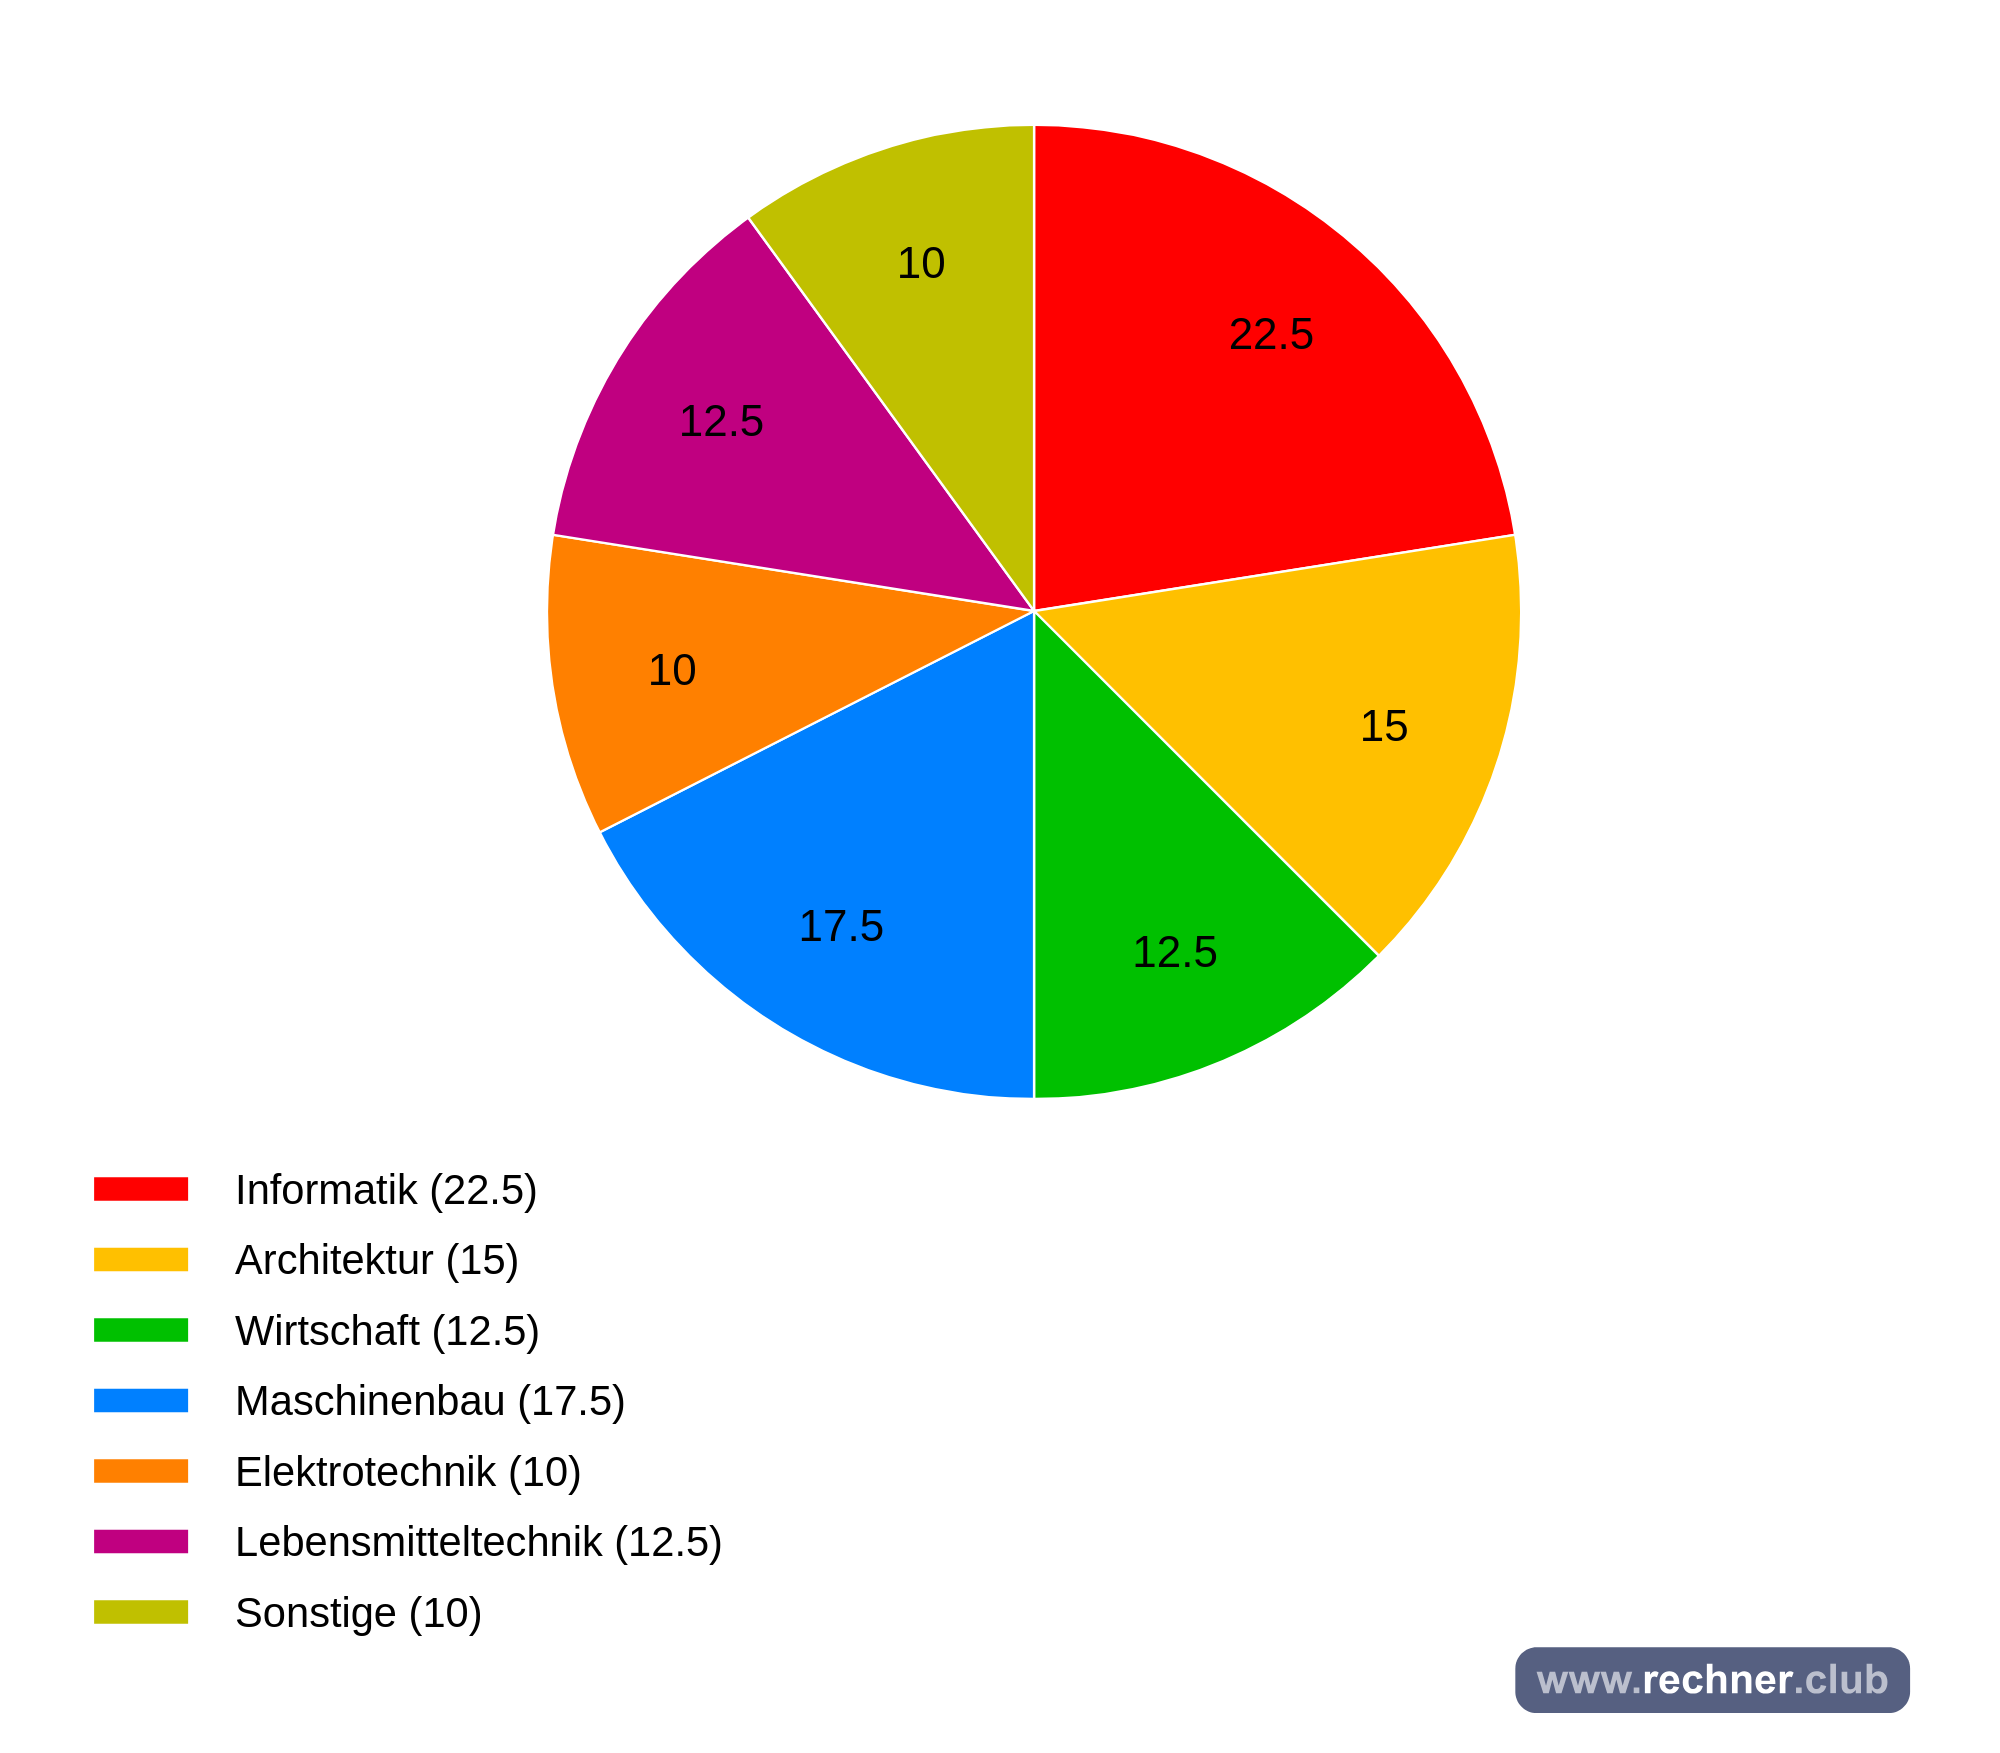
\includegraphics[width=0.8\textwidth]{./assets/abbildung-05-02.png}
        \caption{H"aufigkeit der Studienf"acher (Kreisdiagramm)}
        \label{fig:abbildung-05-02}
    \end{figure}
\end{enumerate}
